
%% bare_conf.tex
%% V1.3
%% 2007/01/11
%% by Michael Shell
%% See:
%% http://www.michaelshell.org/
%% for current contact information.
%%
%% This is a skeleton file demonstrating the use of IEEEtran.cls
%% (requires IEEEtran.cls version 1.7 or later) with an IEEE conference paper.
%%
%% Support sites:
%% http://www.michaelshell.org/tex/ieeetran/
%% http://www.ctan.org/tex-archive/macros/latex/contrib/IEEEtran/
%% and
%% http://www.ieee.org/

%%*************************************************************************
%% Legal Notice:
%% This code is offered as-is without any warranty either expressed or
%% implied; without even the implied warranty of MERCHANTABILITY or
%% FITNESS FOR A PARTICULAR PURPOSE! 
%% User assumes all risk.
%% In no event shall IEEE or any contributor to this code be liable for
%% any damages or losses, including, but not limited to, incidental,
%% consequential, or any other damages, resulting from the use or misuse
%% of any information contained here.
%%
%% All comments are the opinions of their respective authors and are not
%% necessarily endorsed by the IEEE.
%%
%% This work is distributed under the LaTeX Project Public License (LPPL)
%% ( http://www.latex-project.org/ ) version 1.3, and may be freely used,
%% distributed and modified. A copy of the LPPL, version 1.3, is included
%% in the base LaTeX documentation of all distributions of LaTeX released
%% 2003/12/01 or later.
%% Retain all contribution notices and credits.
%% ** Modified files should be clearly indicated as such, including  **
%% ** renaming them and changing author support contact information. **
%%
%% File list of work: IEEEtran.cls, IEEEtran_HOWTO.pdf, bare_adv.tex,
%%                    bare_conf.tex, bare_jrnl.tex, bare_jrnl_compsoc.tex
%%*************************************************************************

% *** Authors should verify (and, if needed, correct) their LaTeX system  ***
% *** with the testflow diagnostic prior to trusting their LaTeX platform ***
% *** with production work. IEEE's font choices can trigger bugs that do  ***
% *** not appear when using other class files.                            ***
% The testflow support page is at:
% http://www.michaelshell.org/tex/testflow/



% Note that the a4paper option is mainly intended so that authors in
% countries using A4 can easily print to A4 and see how their papers will
% look in print - the typesetting of the document will not typically be
% affected with changes in paper size (but the bottom and side margins will).
% Use the testflow package mentioned above to verify correct handling of
% both paper sizes by the user's LaTeX system.
%
% Also note that the "draftcls" or "draftclsnofoot", not "draft", option
% should be used if it is desired that the figures are to be displayed in
% draft mode.
%
\documentclass[conference]{IEEEtran}
% Add the compsoc option for Computer Society conferences.
%
% If IEEEtran.cls has not been installed into the LaTeX system files,
% manually specify the path to it like:
% \documentclass[conference]{../sty/IEEEtran}





% Some very useful LaTeX packages include:
% (uncomment the ones you want to load)


% *** MISC UTILITY PACKAGES ***
%
%\usepackage{ifpdf}
% Heiko Oberdiek's ifpdf.sty is very useful if you need conditional
% compilation based on whether the output is pdf or dvi.
% usage:
% \ifpdf
%   % pdf code
% \else
%   % dvi code
% \fi
% The latest version of ifpdf.sty can be obtained from:
% http://www.ctan.org/tex-archive/macros/latex/contrib/oberdiek/
% Also, note that IEEEtran.cls V1.7 and later provides a builtin
% \ifCLASSINFOpdf conditional that works the same way.
% When switching from latex to pdflatex and vice-versa, the compiler may
% have to be run twice to clear warning/error messages.






% *** CITATION PACKAGES ***
%
%\usepackage{cite}
% cite.sty was written by Donald Arseneau
% V1.6 and later of IEEEtran pre-defines the format of the cite.sty package
% \cite{} output to follow that of IEEE. Loading the cite package will
% result in citation numbers being automatically sorted and properly
% "compressed/ranged". e.g., [1], [9], [2], [7], [5], [6] without using
% cite.sty will become [1], [2], [5]--[7], [9] using cite.sty. cite.sty's
% \cite will automatically add leading space, if needed. Use cite.sty's
% noadjust option (cite.sty V3.8 and later) if you want to turn this off.
% cite.sty is already installed on most LaTeX systems. Be sure and use
% version 4.0 (2003-05-27) and later if using hyperref.sty. cite.sty does
% not currently provide for hyperlinked citations.
% The latest version can be obtained at:
% http://www.ctan.org/tex-archive/macros/latex/contrib/cite/
% The documentation is contained in the cite.sty file itself.






% *** GRAPHICS RELATED PACKAGES ***
%
\ifCLASSINFOpdf
  % \usepackage[pdftex]{graphicx}
  % declare the path(s) where your graphic files are
  % \graphicspath{{../pdf/}{../jpeg/}}
  % and their extensions so you won't have to specify these with
  % every instance of \includegraphics
  % \DeclareGraphicsExtensions{.pdf,.jpeg,.png}
\else
  % or other class option (dvipsone, dvipdf, if not using dvips). graphicx
  % will default to the driver specified in the system graphics.cfg if no
  % driver is specified.
  % \usepackage[dvips]{graphicx}
  % declare the path(s) where your graphic files are
  % \graphicspath{{../eps/}}
  % and their extensions so you won't have to specify these with
  % every instance of \includegraphics
  % \DeclareGraphicsExtensions{.eps}
\fi
% graphicx was written by David Carlisle and Sebastian Rahtz. It is
% required if you want graphics, photos, etc. graphicx.sty is already
% installed on most LaTeX systems. The latest version and documentation can
% be obtained at: 
% http://www.ctan.org/tex-archive/macros/latex/required/graphics/
% Another good source of documentation is "Using Imported Graphics in
% LaTeX2e" by Keith Reckdahl which can be found as epslatex.ps or
% epslatex.pdf at: http://www.ctan.org/tex-archive/info/
%
% latex, and pdflatex in dvi mode, support graphics in encapsulated
% postscript (.eps) format. pdflatex in pdf mode supports graphics
% in .pdf, .jpeg, .png and .mps (metapost) formats. Users should ensure
% that all non-photo figures use a vector format (.eps, .pdf, .mps) and
% not a bitmapped formats (.jpeg, .png). IEEE frowns on bitmapped formats
% which can result in "jaggedy"/blurry rendering of lines and letters as
% well as large increases in file sizes.
%
% You can find documentation about the pdfTeX application at:
% http://www.tug.org/applications/pdftex





% *** MATH PACKAGES ***
%
%\usepackage[cmex10]{amsmath}
% A popular package from the American Mathematical Society that provides
% many useful and powerful commands for dealing with mathematics. If using
% it, be sure to load this package with the cmex10 option to ensure that
% only type 1 fonts will utilized at all point sizes. Without this option,
% it is possible that some math symbols, particularly those within
% footnotes, will be rendered in bitmap form which will result in a
% document that can not be IEEE Xplore compliant!
%
% Also, note that the amsmath package sets \interdisplaylinepenalty to 10000
% thus preventing page breaks from occurring within multiline equations. Use:
%\interdisplaylinepenalty=2500
% after loading amsmath to restore such page breaks as IEEEtran.cls normally
% does. amsmath.sty is already installed on most LaTeX systems. The latest
% version and documentation can be obtained at:
% http://www.ctan.org/tex-archive/macros/latex/required/amslatex/math/





% *** SPECIALIZED LIST PACKAGES ***
%
%\usepackage{algorithmic}
% algorithmic.sty was written by Peter Williams and Rogerio Brito.
% This package provides an algorithmic environment fo describing algorithms.
% You can use the algorithmic environment in-text or within a figure
% environment to provide for a floating algorithm. Do NOT use the algorithm
% floating environment provided by algorithm.sty (by the same authors) or
% algorithm2e.sty (by Christophe Fiorio) as IEEE does not use dedicated
% algorithm float types and packages that provide these will not provide
% correct IEEE style captions. The latest version and documentation of
% algorithmic.sty can be obtained at:
% http://www.ctan.org/tex-archive/macros/latex/contrib/algorithms/
% There is also a support site at:
% http://algorithms.berlios.de/index.html
% Also of interest may be the (relatively newer and more customizable)
% algorithmicx.sty package by Szasz Janos:
% http://www.ctan.org/tex-archive/macros/latex/contrib/algorithmicx/




% *** ALIGNMENT PACKAGES ***
%
%\usepackage{array}
% Frank Mittelbach's and David Carlisle's array.sty patches and improves
% the standard LaTeX2e array and tabular environments to provide better
% appearance and additional user controls. As the default LaTeX2e table
% generation code is lacking to the point of almost being broken with
% respect to the quality of the end results, all users are strongly
% advised to use an enhanced (at the very least that provided by array.sty)
% set of table tools. array.sty is already installed on most systems. The
% latest version and documentation can be obtained at:
% http://www.ctan.org/tex-archive/macros/latex/required/tools/


%\usepackage{mdwmath}
%\usepackage{mdwtab}
% Also highly recommended is Mark Wooding's extremely powerful MDW tools,
% especially mdwmath.sty and mdwtab.sty which are used to format equations
% and tables, respectively. The MDWtools set is already installed on most
% LaTeX systems. The lastest version and documentation is available at:
% http://www.ctan.org/tex-archive/macros/latex/contrib/mdwtools/


% IEEEtran contains the IEEEeqnarray family of commands that can be used to
% generate multiline equations as well as matrices, tables, etc., of high
% quality.


%\usepackage{eqparbox}
% Also of notable interest is Scott Pakin's eqparbox package for creating
% (automatically sized) equal width boxes - aka "natural width parboxes".
% Available at:
% http://www.ctan.org/tex-archive/macros/latex/contrib/eqparbox/





% *** SUBFIGURE PACKAGES ***
%\usepackage[tight,footnotesize]{subfigure}
% subfigure.sty was written by Steven Douglas Cochran. This package makes it
% easy to put subfigures in your figures. e.g., "Figure 1a and 1b". For IEEE
% work, it is a good idea to load it with the tight package option to reduce
% the amount of white space around the subfigures. subfigure.sty is already
% installed on most LaTeX systems. The latest version and documentation can
% be obtained at:
% http://www.ctan.org/tex-archive/obsolete/macros/latex/contrib/subfigure/
% subfigure.sty has been superceeded by subfig.sty.



%\usepackage[caption=false]{caption}
%\usepackage[font=footnotesize]{subfig}
% subfig.sty, also written by Steven Douglas Cochran, is the modern
% replacement for subfigure.sty. However, subfig.sty requires and
% automatically loads Axel Sommerfeldt's caption.sty which will override
% IEEEtran.cls handling of captions and this will result in nonIEEE style
% figure/table captions. To prevent this problem, be sure and preload
% caption.sty with its "caption=false" package option. This is will preserve
% IEEEtran.cls handing of captions. Version 1.3 (2005/06/28) and later 
% (recommended due to many improvements over 1.2) of subfig.sty supports
% the caption=false option directly:
%\usepackage[caption=false,font=footnotesize]{subfig}
%
% The latest version and documentation can be obtained at:
% http://www.ctan.org/tex-archive/macros/latex/contrib/subfig/
% The latest version and documentation of caption.sty can be obtained at:
% http://www.ctan.org/tex-archive/macros/latex/contrib/caption/




% *** FLOAT PACKAGES ***
%
%\usepackage{fixltx2e}
% fixltx2e, the successor to the earlier fix2col.sty, was written by
% Frank Mittelbach and David Carlisle. This package corrects a few problems
% in the LaTeX2e kernel, the most notable of which is that in current
% LaTeX2e releases, the ordering of single and double column floats is not
% guaranteed to be preserved. Thus, an unpatched LaTeX2e can allow a
% single column figure to be placed prior to an earlier double column
% figure. The latest version and documentation can be found at:
% http://www.ctan.org/tex-archive/macros/latex/base/



%\usepackage{stfloats}
% stfloats.sty was written by Sigitas Tolusis. This package gives LaTeX2e
% the ability to do double column floats at the bottom of the page as well
% as the top. (e.g., "\begin{figure*}[!b]" is not normally possible in
% LaTeX2e). It also provides a command:
%\fnbelowfloat
% to enable the placement of footnotes below bottom floats (the standard
% LaTeX2e kernel puts them above bottom floats). This is an invasive package
% which rewrites many portions of the LaTeX2e float routines. It may not work
% with other packages that modify the LaTeX2e float routines. The latest
% version and documentation can be obtained at:
% http://www.ctan.org/tex-archive/macros/latex/contrib/sttools/
% Documentation is contained in the stfloats.sty comments as well as in the
% presfull.pdf file. Do not use the stfloats baselinefloat ability as IEEE
% does not allow \baselineskip to stretch. Authors submitting work to the
% IEEE should note that IEEE rarely uses double column equations and
% that authors should try to avoid such use. Do not be tempted to use the
% cuted.sty or midfloat.sty packages (also by Sigitas Tolusis) as IEEE does
% not format its papers in such ways.





% *** PDF, URL AND HYPERLINK PACKAGES ***
%
%\usepackage{url}
% url.sty was written by Donald Arseneau. It provides better support for
% handling and breaking URLs. url.sty is already installed on most LaTeX
% systems. The latest version can be obtained at:
% http://www.ctan.org/tex-archive/macros/latex/contrib/misc/
% Read the url.sty source comments for usage information. Basically,
% \url{my_url_here}.





% *** Do not adjust lengths that control margins, column widths, etc. ***
% *** Do not use packages that alter fonts (such as pslatex).         ***
% There should be no need to do such things with IEEEtran.cls V1.6 and later.
% (Unless specifically asked to do so by the journal or conference you plan
% to submit to, of course. )


% correct bad hyphenation here
\hyphenation{op-tical net-works semi-conduc-tor}
\usepackage{graphicx}
\begin{document}
\DeclareGraphicsExtensions{png}

%
% paper title
% can use linebreaks \\ within to get better formatting as desired
\title{IN4392: Automatic resource management of Python web applications at Amazon Web Services}


% author names and affiliations
% use a multiple column layout for up to three different
% affiliations
\author{\IEEEauthorblockN{Mircea Cadariu}
\IEEEauthorblockA{EEMCS Faculty\\
Delft University of Technology\\
Email: M.Cadariu@student.tudelft.nl}
\and
\IEEEauthorblockN{Zmicier Zaleznicenka}
\IEEEauthorblockA{EEMCS Faculty\\
Delft University of Technology\\
Email: D.V.Zhaleznichenka@student.tudelft.nl}}

% conference papers do not typically use \thanks and this command
% is locked out in conference mode. If really needed, such as for
% the acknowledgment of grants, issue a \IEEEoverridecommandlockouts
% after \documentclass

% for over three affiliations, or if they all won't fit within the width
% of the page, use this alternative format:
% 
%\author{\IEEEauthorblockN{Michael Shell\IEEEauthorrefmark{1},
%Homer Simpson\IEEEauthorrefmark{2},
%James Kirk\IEEEauthorrefmark{3}, 
%Montgomery Scott\IEEEauthorrefmark{3} and
%Eldon Tyrell\IEEEauthorrefmark{4}}
%\IEEEauthorblockA{\IEEEauthorrefmark{1}School of Electrical and Computer Engineering\\
%Georgia Institute of Technology,
%Atlanta, Georgia 30332--0250\\ Email: see http://www.michaelshell.org/contact.html}
%\IEEEauthorblockA{\IEEEauthorrefmark{2}Twentieth Century Fox, Springfield, USA\\
%Email: homer@thesimpsons.com}
%\IEEEauthorblockA{\IEEEauthorrefmark{3}Starfleet Academy, San Francisco, California 96678-2391\\
%Telephone: (800) 555--1212, Fax: (888) 555--1212}
%\IEEEauthorblockA{\IEEEauthorrefmark{4}Tyrell Inc., 123 Replicant Street, Los Angeles, California 90210--4321}}




% use for special paper notices
%\IEEEspecialpapernotice{(Invited Paper)}




% make the title area
\maketitle


\begin{abstract}
%\boldmath
This paper discusses a system intended for the automatic deployment and monitoring of Python web applications using Amazon Web Services infrastructure. The proposed system was developed as a lab assignment for IN4392 Cloud Computing course at TU Delft. The functionality of a system resembles Elastic Beanstalk service provided by Amazon though the discussed system has less functionality. The performed evaluation shows that AWS is a reliable cloud computing platform for hosting applications of virtually arbitrary complexity.
\end{abstract}
% IEEEtran.cls defaults to using nonbold math in the Abstract.
% This preserves the distinction between vectors and scalars. However,
% if the conference you are submitting to favors bold math in the abstract,
% then you can use LaTeX's standard command \boldmath at the very start
% of the abstract to achieve this. Many IEEE journals/conferences frown on
% math in the abstract anyway.

% no keywords




% For peer review papers, you can put extra information on the cover
% page as needed:
% \ifCLASSOPTIONpeerreview
% \begin{center} \bfseries EDICS Category: 3-BBND \end{center}
% \fi
%
% For peerreview papers, this IEEEtran command inserts a page break and
% creates the second title. It will be ignored for other modes.
\IEEEpeerreviewmaketitle



\section{Introduction}

In recent years cloud computing became a hot and emerging topic both in industry and academia. A large amount of cloud providers offer now their computational capacities for reasonable prices and the services offered in the clouds gain more and more popularity. Cloud computing platforms have many advantages over the traditional approaches in building infrastructure for the IT projects like purchasing own hardware, leasing it from data centers or utilizing the capacities of computational grids. These advantages include elasticity, high capacity, redundancy, ease of maintenance, flexible payment schemas and more. 

Apart from providing pure computational power and virtually unlimited storage on demand, the cloud providers usually give their customers access to the additional services intended to automate the daily tasks of the system administrators working with the cloud platform. These services may add such functionality as automatic scaling, load balancing, real-time monitoring and e-mail notifications. Thus, one of the leading cloud computing providers Amazon Web Services (AWS) by the time this paper is being written supports over 25 services augmenting its major Simple Storage Service (S3) and Elastic Compute Cloud (EC2) services. 

One of the important problems for the engineers willing to deploy their applications at AWS and similar cloud computing platforms is the need to get acquainted with all the diversity of services available at their cloud provider to work efficiently. While the large companies may afford having a dedicated specialist or a whole team busy with establishing and maintaining cloud infrastructure, for independent developers or small engineering or research groups this is usually impossible. Such teams want to benefit from all the advantages offered by the additional services in the cloud and spend as little time as possible in studying the proper ways to work with them in the meantime.

One of the solutions to this problem is the introduction of an additional service that would be used for rapid creation and easy management of rich environments utilizing most of the services available at the given cloud provider. Such a service should have a relatively small number of options and easy API allowing the developers to start working with the services offered by their cloud provider almost immediately. 

AWS has its own service that is responsible for rapid application deployment. It is called Elastic Beanstalk (EB) and it allows to deploy .Net, Java, PHP, Python and Ruby applications at AWS premises in minutes. The applications deployed with EB benefit from immediately available detailed monitoring, e-mail notifications, a number of database services, auto-scaling and more. The similar services are also offered by many third parties, like RightScale\footnote{http://www.rightscale.com} or Scalarium\footnote{http://www.scalarium.com}. An additional benefit of these services is the support of many cloud providers. This means that if an engineering team decides to change their provider, they do not need to study the services offered by their new supplier as the only thing needed is to update the configuration of the intermediary service.

The project described in this paper was conducted as a lab assignment for IN4392 Cloud Computing course at TU Delft, The Netherlands and is an attempt to implement a service similar to AWS EB which should allow software developers to deploy and monitor Python web applications at AWS cloud. The implemented system is less advanced that EB. Due to the lab requirements it does not utilize APIs of many AWS services but provides an own implementation of them instead. The course was taught by dr. D.H.J. Epema and dr. A. Iosup, the lab work was supervised by B. Ghit (\{D.H.J.Epema,A.Iosup,B.I.Ghit\}@tudelft.nl).

The source code of this project and the latest version of this report are publicly available on Github\footnote{https://github.com/dzzh/IN4392}.

The remainder of this paper is organized as follows. Section 2 contains a description of a reference web application built to test the forthcoming system. Section 3 discusses the system design and policies. Section 4 contains the evaluation. Section 5 is a discussion of general cloud computing platform properties and trade-offs. Section 6 contains suggestions for the future work. Section 7 reports the conclusions.

% An example of a floating figure using the graphicx package.
% Note that \label must occur AFTER (or within) \caption.
% For figures, \caption should occur after the \includegraphics.
% Note that IEEEtran v1.7 and later has special internal code that
% is designed to preserve the operation of \label within \caption
% even when the captionsoff option is in effect. However, because
% of issues like this, it may be the safest practice to put all your
% \label just after \caption rather than within \caption{}.
%
% Reminder: the "draftcls" or "draftclsnofoot", not "draft", class
% option should be used if it is desired that the figures are to be
% displayed while in draft mode.
%
%\begin{figure}[!t]
%\centering
%\includegraphics[width=2.5in]{myfigure}
% where an .eps filename suffix will be assumed under latex, 
% and a .pdf suffix will be assumed for pdflatex; or what has been declared
% via \DeclareGraphicsExtensions.
%\caption{Simulation Results}
%\label{fig_sim}
%\end{figure}

% Note that IEEE typically puts floats only at the top, even when this
% results in a large percentage of a column being occupied by floats.


% An example of a double column floating figure using two subfigures.
% (The subfig.sty package must be loaded for this to work.)
% The subfigure \label commands are set within each subfloat command, the
% \label for the overall figure must come after \caption.
% \hfil must be used as a separator to get equal spacing.
% The subfigure.sty package works much the same way, except \subfigure is
% used instead of \subfloat.
%
%\begin{figure*}[!t]
%\centerline{\subfloat[Case I]\includegraphics[width=2.5in]{subfigcase1}%
%\label{fig_first_case}}
%\hfil
%\subfloat[Case II]{\includegraphics[width=2.5in]{subfigcase2}%
%\label{fig_second_case}}}
%\caption{Simulation results}
%\label{fig_sim}
%\end{figure*}
%
% Note that often IEEE papers with subfigures do not employ subfigure
% captions (using the optional argument to \subfloat), but instead will
% reference/describe all of them (a), (b), etc., within the main caption.


% An example of a floating table. Note that, for IEEE style tables, the 
% \caption command should come BEFORE the table. Table text will default to
% \footnotesize as IEEE normally uses this smaller font for tables.
% The \label must come after \caption as always.
%
%\begin{table}[!t]
%% increase table row spacing, adjust to taste
%\renewcommand{\arraystretch}{1.3}
% if using array.sty, it might be a good idea to tweak the value of
% \extrarowheight as needed to properly center the text within the cells
%\caption{An Example of a Table}
%\label{table_example}
%\centering
%% Some packages, such as MDW tools, offer better commands for making tables
%% than the plain LaTeX2e tabular which is used here.
%\begin{tabular}{|c||c|}
%\hline
%One & Two\\
%\hline
%Three & Four\\
%\hline
%\end{tabular}
%\end{table}


% Note that IEEE does not put floats in the very first column - or typically
% anywhere on the first page for that matter. Also, in-text middle ("here")
% positioning is not used. Most IEEE journals/conferences use top floats
% exclusively. Note that, LaTeX2e, unlike IEEE journals/conferences, places
% footnotes above bottom floats. This can be corrected via the \fnbelowfloat
% command of the stfloats package.
\section{Background on application}

Considering the time limitations for the project implementation, it was decided not to develop a very general service supporting many languages and frameworks available for the deployment but rather restrict to a particular class of the applications. Thus, the discussed system supports web applications written in Python and managed by Apache web server with mod\_wsgi installed.

Before working on the infrastructural services responsible for AWS interaction, we have implemented a simple web service to be used as a reference web application for AWS environment. We have chosen matrices multiplication operation to be provided by the reference application as this operation can be implemented in a straightforward way and requires a lot of computational resources for completion thus allowing to perform load testing easily.

The reference application has simple user interface allowing a client to choose matrices dimension to multiply and start the computation. Before starting the computation, two random square matrices of given dimension are generated. After the computation is completed, the client is shown a web page with the time spent on computation. The results of the multiplication are not stored and if a user issues a new request, the whole computation is performed again with the newly generated matrices.

\section{System design}
\subsection{Resource management architecture}
IN4392 system consists of three main parts, namely Environment manager, System monitor and Monitoring GUI. All of these components run at a client machine and do not need in allocating any resources in the cloud for their proper operation.

Environment manager is responsible for creating and deleting the AWS environments. In the terms of this project an environment means a virtual organization of running and stopped instances that have the same application deployed and a load balancer which is used to direct client requests to one of the running computational instances.

A user of IN4392 starts working with the system by creating an environment using the Environment manager. While creating an environment, a minimal number of instances required for its proper operation is created at AWS data center. After the instances are launched, Environment manager starts an instance of AWS Elastic Load Balancer (ELB) and attaches the computational instances to it. In addition, at this stage the Environment manager sets up a security group and establishes test connection with the instance to ensure it started correctly.

When the environment is created, a client should ask Environment manager to deploy his application to it. At this stage, the client application and the instance configuration files get transferred to AWS instances. Environment manager connects to the instances using SSH protocol and performs the required management tasks to set up the application and start a web server. After this stage is done, the application becomes available online and may accept the incoming HTTP connections. 

When the client does not need in an environment anymore, he can use Environment manager to delete it. When deleting the environment, all the computational instances and ELB instance terminate.

System monitor has to be started by the client after the application is deployed. The monitor is implemented as a script running an endless loop. It is responsible for auto scaling, health checks and informing about CPU utilization at the running computational instances. The System monitor adds to the system all the basic features that are requested in the assignment description. These features are implemented as follows.

After the monitor is started, no additional user interaction is needed for its proper operation. The System monitor constantly analyzes the state of a system and makes decisions based on the data retrieved from AWS CloudWatch (CW) monitoring service and the system configuration. This was the requirement for the \emph{Automation} feature. 

\emph{Elasticity} and \emph{Performance} requirements are addressed with the auto-scaling part of the System monitor. When the system needs to scale up, it looks for the available VMs in the resource pool. If the pool is not empty, one VM from it gets started. Otherwise a new VM is started and the application gets deployed to it. If the system exceeds the maximum number of VMs allowed to be run simultaneously, System monitor issues a warning. When down-scaling, one of the running instances is stopped and placed into the resource pool until reaching the minimum number of running instances.

Each VM may have only one application instance running but the number of allowed simultaneous WSGI processes and threads inside the VM can be adjusted in the system configuration.

\emph{Reliability} feature is implemented with the health check procedure in the System monitor. In each monitoring iteration, the monitor requests the load balancer for the current state of its instances. If any of the instances reports any errors for several consequent checks, it gets stopped and the monitor logs this event. Later, a new instance is automatically added instead of the unhealthy one during the auto-scaling check.

The existence of the monitoring service itself solves the \emph{Monitoring} requirement. So far, the functionality available in the Service monitor allows only to monitor the CPU utilization at the environment and certain computational instances, but it can be easily expanded. In addition, Monitoring GUI component provides visualization data for the environment CPU utilization. 

Monitoring GUI is used to visualize the aspects that define the behavior of the application. This tool can be used to analyze the evolution of CPU utilization for the running instances of the computational environment. The data is displayed in a form of time-series chart, therefore the user can observe the trends in CPU utilization of the environment instances. 

Monitoring GUI is implemented as MVC application where the Model part is written as queries to AWS CW service, the Controllers are the Python wrappers that encapsulate queries to CloudWatch and serve the requests coming from the user via the browser and the Views are the web pages 
where the user can see charts and issue requests for their update. 

IN4392 system has a number of configuration options that can be either default or specific for the given environments. The decisions made by Environment manager and System monitor are based on the application configuration and can be easily adjusted. All the components of the system are tightly integrated and reuse the code wherever possible. 

\subsection{System policies}

The system currently supports two system policies applied to the System monitor operations. The first policy is related to the size of the resource pool. The system allows the user to specify minimum and maximum number of computational instances that can be run concurrently. The minimum limit is needed to guarantee certain system performance, the maximum limit is used to control the spendings on the environment.

The second policy defines CPU utilization limits used for auto-scaling. When the utilization falls below the lower limit, the monitor makes decision to scale down. Reciprocally, when the utilization exceeds the upper limit, the monitor makes decision to scale up. 

The current version of the System monitor is rather simple and straightforward to support the additional system policies, but if it is improved for monitoring the other metrics, the respective system policies can be added to it.

\subsection{Additional system features}

While working on the project some effort was put into implementing \emph{Security} and \emph{Benchmarking} additional requirements.

The \emph{Security} requirement is solved by applying the EC2 security groups policies while launching new computational instances. Currently, the security policy applied to the instance allows only HTTP and SSH access to it. For SSH access it is required to have private key file in possession. 

Security can be improved further by adjusting the security policy after the instance is launched. When all the maintenance operations with it are done, there is no more need to keep SSH port opened and the respective rule can be removed from the policy. However, due to the time pressure this has not been implemented.

A number of tests were created in Apache JMeter tool for analyzing the behavior of the system under the peak load and verify the correctness of System monitor implementation. The existence of these tests and their description in the consequent chapter address the \emph{Benchmarking} requirement.

\section{Experimental results}

\subsection{Experimental setup}

All the experiments discussed in this section were conducted at the environments created with IN4392 system in Ireland region of AWS cloud. The reference application discussed in Section 2 was deployed on a number of t1.micro AWS instances and used ami-6d555119 VM (64-bit Amazon Linux with Python 2.6) and Apache 2.2 web server. The environment was configured to use at least one and at most five computational instances simultaneously.

No specific automated tests were written to test the Environment manager component. Instead, a thorough manual testing was performed after its implementation to make sure the manager correctly creates and deletes the environments as well as deploys the reference application to the launched computational instances.

While testing the Environment manager, the results of its work were validated against the output of the AWS management console. The correct application deployment procedure was verified by opening the launched application in the browser, interacting with it through the UI and analyzing web server logs. 

To test the behavior of System monitor, a number of test plans were created using Apache JMeter\footnote{http://jmeter.apache.org} load testing tool. Each JMeter test is represented as a sequence of thread groups connecting to the ELB instance balancing the load of the environment and requesting the application to multiply two 100x100 random matrices. At different stages, various number of simultaneous threads and requests per thread are used to simulate different load and test the correctness of the System monitor, namely its ability to react on computational instance failures and need in auto-scaling.

For the tests, up-scaling CPU utilization limit was set to 90\%, down-scaling limit was set to 40\%. Minimum number of running instances was set to 1, maximum number was set to 5.

Monitoring GUI was tested manually. CPU Utilization graphs available from it were compared with the graphs provided at AWS CW console.

IN4392 system is fully implemented in Python programming language. For interacting with AWS, boto\footnote{https://github.com/boto/boto} framework was used. Data visualization at Monitoring GUI component is generated using Google Visualization Python API\footnote{http://code.google.com/p/google-visualization-python/}. To create web applications (both reference matrix multiplication application and Monitoring GUI), web.py\footnote{http://webpy.org} framework was used. Twitter Bootstrap\footnote{http://twitter.github.com/bootstrap/} was used as UI library for the reference web application.

\subsection{Experiments}

\subsubsection{7-stage JMeter test description}

For the purposes of thorough testing of a System monitor and analyzing the system behavior under various loads, a seven-stage JMeter test plan was created. Its parameters are presented in Table \ref{table-test-parameters}. The results of its execution are provided at Figure 1.

\begin{table}[ht]
\begin{center}
  \begin{tabular}{ | c | c | c | c | }
    \hline
    \textbf{Stage} & \textbf{Threads} & \textbf{Samples/Thread} & \textbf{Delay} \\ \hline
    1 & 2 & 500 & 5000 \\ \hline
    2 & 5 & 300 & 3000 \\ \hline
    3 & 1 & 500 & 5000 \\ \hline
    4 & 10 & 200 & 2000 \\ \hline
    5 & 2 & 500 & 5000 \\ \hline
    6 & 10 & 150 & 2000 \\ \hline
    7 & 1 & 170 & 10000 \\
    \hline
  \end{tabular}
  \caption{7-stage JMeter test parameters.}
  \label{table-test-parameters}
\end{center}
\end{table}

\begin{figure*}
\centering
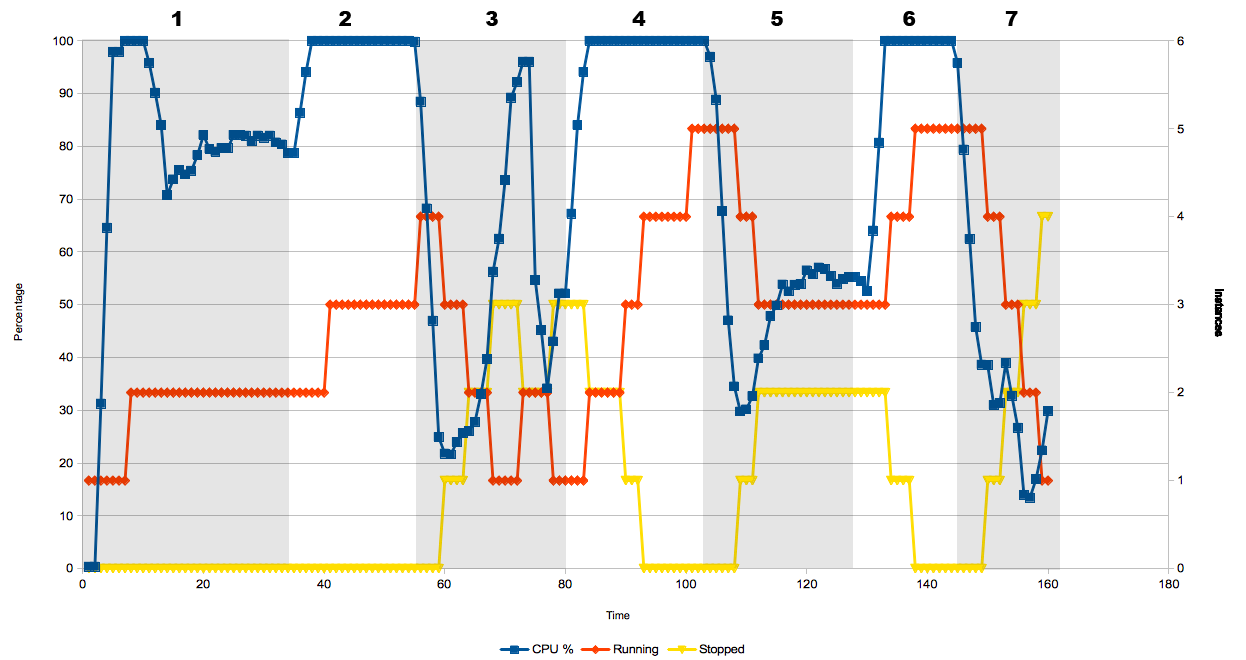
\includegraphics[width=180mm]{big_chart.png}
\caption{Execution results for 7-stage JMeter test.}
\label{fig_sim}
\end{figure*}

At each testing stage, different number of threads were run concurrently, each performing N requests to the load balancer. Between two consequent requests, a thread was delayed for random time, with maximum delay in milliseconds reported in Table \ref{table-test-parameters}.

The first stage was designed to be a warm-up, with just two threads and quite large delay between the requests. During the second stage, the load was increased by introducing three more threads and reducing the delay. Stage 3 was introduced to decrease the load to its very minimum and thus test the down-scaling functionality of System monitor. Stage 4 was a stress test exceeding the capabilities of the system. It was planned that all the available instances would start and the monitor would warn the user about the system overloading. Stage 5 was a relaxation with just 2 threads running. Stage 6 was another stress test testing the VMs allocation from the resource pool. Stage 7 was the final down-scaling stage testing that the environment is able to scale down to one single running instance.

These different execution stages are marked at the top of Figure 1 and can be distinguished by different background colors. The figure contains three graphs. Blue line shows the CPU usage of the environment in percents, red line shows the number of running instances and yellow line shows the number of stopped instances. Time is measured in minutes. 

\subsubsection{7-stage JMeter test analysis}

From the testing results, the following conclusions can be made. We see that during the first stage, the system was under high load and had to scale up by one instance. This means that the selected reference application consumes available CPU resources very aggressively. After the load was increased to five threads, the system scaled up to four running instances. We see, that between two upscaling events almost 15 minutes passed. The length of this period is caused by two factors. First of all, after the system reports that it has scaled up, a new instance does not accept new connections for a couple of minutes while being registered at the load balancer. Then, the monitor waits for AWS CW service to start sending monitoring statistics for the new instance. In some situation, this happens fast (see upscaling events around minutes 92 and 100), sometimes this lag is longer. This means that the system is not able to react to the changes in the load patterns quickly, time lag is always present and it may take up to 15 minutes (or even more) between two upscaling events.

It can also be seen that the upscaling event at minute 56 was reported when the system had already switched to stage 3. This is related to the fact that upscaling process takes around two minutes for instance launch and application deployment. The system reports that upscaling is completed when a new instance is already running and attached to the load balancer, but the signal for it to launch is usually issued around two minutes earlier. For the instances running from the pool, the launching period was approximately one minute long.

At stage 3 we see that the system becomes underloaded and within ten minutes there are three down-scaling events. The smallest period between two auto-scaling events can be configured in the application settings to prevent the monitor from very frequent changes in the environment structure, to scale up and scale down gradually and have enough time for the system analysis between the auto-scaling events. 

After scaling down to one instance, during stage 3 the system upscales and downscales back. To prevent it from such behavior, a lower down-scaling CPU utilization limit has to be set. It was set to 40\% to see more auto-scaling events in this test. In production, this limit can be set to 20\% CPU utilization or even lower.

During stage 4 we see that the utilization is raised up to 100\% and remained there till this stage ends. During this time, the system gradually scales up, first from the pool of the stopped instances, then by initiating the new instances until it exceeds maximum number of them. When it is done (around minute 100), the system writes warnings to the log file, informing the user that further upscaling is needed.

At stage 5 the system gradually scales down to three running instances. Two instances get stopped and become available in the pool. During stage 6, the system scales up again and reports about the need to scale up further. During stage 7 it gradually scales down and places four stopped instances at the pool. 

Generally, the performed load test have shown that the reference application selection was not entirely correct as matrix multiplication operation consumes resources in a different way than most web applications do. Mathematical operations quickly load the processor by 100\% and it is difficult to execute similar operations at a single-core machine in parallel efficiently. Thus, even one user issuing requests to the server may load it by 100\% quickly. On the other hand, many typical web applications are rather I/O-bound than CPU-bound (due to simple computational logic and database queries) and may be executed at a single-core computational instance simultaneously by many parallel threads while keeping CPU utilization low.

Another conclusion from the load test is that the monitoring service provided by AWS is not able to gather the data from the instances in real-time, in most situations the results were provided with a lag of 1-2 minutes. This lag has to be considered while designing the auto-scaling strategy and it is needed to know that it is impossible to up-scale the application immediately. At least several minutes are needed from the environment to understand that the application is overloaded, apply the auto-scaling policy and wait for the instance start-up and its registration at the load balancer. Thus, if an application has weakly predictable load patterns, it is better to keep more running instances that is needed at the moment to diminish the effect of start-up lag.

Time-cost analysis for 7-stage JMeter test is provided in Table \ref{table-test-cost}. From this analysis it is evident that due to the hourly charging system at AWS there is no need to scale the instances down until they work till the end of a full hour. This may even lead to cost savings for certain auto-scaling patterns if comparing with the policy when the instances are scaled down immediately after the load is decreased below the threshold.

\begin{table}[ht]
\begin{center}
  \begin{tabular}{| c | c | c | c | c |}
    \hline
    \textbf{Inst.} & \textbf{Runtime,min} & \textbf{Launches} & \textbf{Charged time,hrs} & \textbf{Cost,USD} \\ \hline
    1 & 160 & 1 & 3 & 0.06 \\ \hline
    2 & 145 & 3 & 5 & 0.1 \\ \hline
    3 & 92 & 2 & 3 & 0.06 \\ \hline
    4 & 48 & 3 & 3 & 0.06 \\ \hline
    5 & 24 & 2 & 2 & 0.04 \\ \hline
    \textbf{total} & \textbf{469} & \textbf{11} & \textbf{16} & \textbf{0.32} \\
    \hline
  \end{tabular}
  \caption{7-stage JMeter test cost.}
  \label{table-test-cost}
\end{center}
\end{table}

\subsubsection{Testing basic system requirements}

With the help of the described test it was possible to analyze most of the basic features required from the system. \emph{Automation} was reached as no human intervention was needed during the test. It was only needed to run a short shell script to create an environment, deploy the application to it, start JMeter and System monitor and delete the environment when the test was done.

\emph{Elasticity} and \emph{Performance} were tested by applying different load patterns to the environment. From the test results we see that the monitor was able to launch the new VMs, stop them and add them back from a resource pool upon a need by a predictable pattern based on the CPU utilization of the environment. \emph{Monitoring} was tested by analyzing the behavior of System monitor and its logs. From them it is clear that the monitor was constantly checking the environment load and reacted accordingly.

For \emph{Reliability} requirement, a simple one-stage stress test was created in JMeter. After this test was started and a number of instances were launched, one instance was manually rebooted via AWS management console. The System monitor reported this event and stopped the instance. A new instance was later added to the environment during normal auto-scaling process.

\section{Discussion}

Cloud computing platforms are being used for several years already for provision of computational power and storage services for different applications, including very large and complex ones. During this time, some cloud providers proved to be reliable suppliers for IaaS solutions, some did not, but the current level of technological development reached in the best and the most expensive data centers available for cloud computing customers allows to host there the applications of virtually arbitrary complexity with satisfactory service level guarantees. 

When deciding whether to place an application at the data center of a cloud provider, a number of issues have to be taken into account. These issues may be categorized into financial and technological. 

Placement of the application in the cloud has its advantages and disadvantages both for financial and technological aspects. From financial point of view, a definite advantage of leasing the resources from the cloud is the elimination of high upfront expenses on building the own service infrastructure and paying high salaries for its support staff from the very beginning of the project lifecycle. For many of the projects being created while this report is filled in (i.e. deeply in the night), especially for the trendy start-ups raising venture investments it is difficult to predict the popularity of the final product and plan the infrastructural expenses in advance. Cloud computing platforms allow their customers to pay for what they use and adjust their environments in minutes if any errors were made during the planning stage. A disadvantage of cloud computing platforms is that for large long-term projects with predictable load patterns their placement in the cloud is generally more expensive than creating the own service infrastructure. There are some cloud providers that offer rather low rates but it is not always safe to place 100\%-availability-dependent applications there due to their lower fault tolerance and guarantees if comparing with the leaders of the market.

From technological prospect, cloud platforms have a number of interesting properties that are difficult to achieve if having all the infrastructure on the own premises or built into general-purpose data centers. However, these platforms also have their drawbacks.

One of the important cloud platforms advantage already mentioned while discussing the financial aspects is their elasticity. If a customer plans to release a new application to the market and make an advertising campaign for it, it is almost impossible to predict its popularity and the load patterns. Cloud platforms allow to scale literally on-the-fly thus helping system administrators to struggle with extremely high load or to reduce amount of work if the load is low.

Another advantage of IaaS solutions is possibility to deploy global applications near to the end customers. Some of cloud computing providers, e.g. AWS, have their data centers located all over the world and a system administrator can easily manage his environments in different regions using same software or API calls. If building a platform at application vendor premises, its proximity to the end customers is often simply not achievable though it can be an important requirement for some classes of applications, i.e. online games servers which are very susceptible to network latencies by design.

Also, the cloud platforms provide certain service level guarantees that are hard to achieve at the local data centers. For instance, each AWS region has a number of availability zones, with each zone placed at its own premises having different power and network connectivity suppliers. Thus, even in case of serious natural or technological disasters there is possibility that at least some of the availability zones will remain in service. AWS allows to share the computational instances supporting one application within different availability zones in one region thus providing potentially best failure tolerance guarantees possible.

The technological disadvantages of using IaaS solutions are the following. First of all, the available hardware is usually limited by rather small number of configurations and it is impossible for the customers to build an own configuration that would serve their needs in the best way. Secondly, cloud computing platforms usually provide access not to hardware itself but to the virtual machines launched on top of it which may sometimes impose problems with the declared performance of the computational instances. The new instances may be added to the resource pools from different racks which can be inappropriate for the applications requiring high inter-node throughput. There are some solutions nowadays when it is possible to lease real hardware instances and guarantee the proximity of the newly added instances but such options are usually very expensive if comparing with having own racks in a general-purpose data center.

It can be concluded that the decision on whether to design an application for deployment at IaaS provider premises or in some other way should be based on a number of financial and technological considerations. In this section we have listed just a few of them but there are more. Large and small application with different usage patterns are successfully hosted in the clouds, in general-purpose data centers and at vendors' premises nowadays which means that there is no general advice that can be given about the selection of a hosting provider without the knowledge of the application requirements and a thorough financial analysis.

We did not perform the cost computations for the reference web application aimed to serve up to 10 000 000 of users as for this application this sort of planning is inappropriate. To analyze the spendings for this amount of customers there is a need to develop another application that would better resemble the load patterns usual for typical high-loaded multi-user applications in the Internet.

\section{Future work}

The application built for IN4392 course can already help its users with deploying Python application at AWS clusters and monitoring their state almost in real-time but many improvements can still be made to it. One of such improvements is the addition of S3 support. With S3, it will be possible to launch new instances in approximately thirty seconds instead of approximately two minutes needed for the launch now as there will be no need to transfer files there from a local machine and wait for the SSH connection to be established. Instead, all the configuration could be done using init scripts. Also, this will allow to make the environment more secure, as there will be no need to keep SSH port open anymore.

Another important improvement to be done for IN4392 is addition of versioning support. Now, it is impossible to deploy a new version of the application to all the computational instances without terminating the environment though this functionality will definitely be required by the end customers, if any.

Also, the system would benefit from the integration with AWS Simple Notification Service (SNS) to inform the administrators about certain events via email, not only logging the warnings to the files.

\section{Conclusion}

During the lab project for IN4392 course we have developed a system allowing to deploy Python web applications developed to use with Apache web server at AWS cloud computing platform. The performed evaluation shows that the built system is able to correctly create and terminate the computational environments as well as to monitor their state while they are in service and react to a number of events thus helping system administrators to manage AWS computational instances. 

AWS is a reliable cloud computing platform with a rich set of services and a number of easy-to-use APIs that allow to deploy applications of virtually arbitrary complexity. It can be recommended as a powerful and flexible IaaS solution.

% conference papers do not normally have an appendix

\appendix

\subsection{Time sheets}

The time sheets as requested can be found in Table \ref{table-timesheets}.
\begin{table}[ht]
\begin{center}
  \begin{tabular}{ | l | c | c | }
    \hline
    \textbf{Time} & \textbf{Mircea} & \textbf{Zmicier} \\ \hline
    total-time & 60 & 76 \\ \hline
    think-time & 15 & 3 \\ \hline
    dev-time & 30 & 2 (ref. app.), 30 (aws scripts) \\ \hline
    xp-time & 0 & 1 (building tests), 14 (testing) \\ \hline
    analysis-time & 0 & 3 \\ \hline
    write-time & 5 & 8 \\ \hline
    wasted-time & 10 & 15 (playing with Elastic Beanstalk) \\
    \hline
  \end{tabular}
  \caption{Time sheets.}
  \label{table-timesheets}
\end{center}
\end{table}

% trigger a \newpage just before the given reference
% number - used to balance the columns on the last page
% adjust value as needed - may need to be readjusted if
% the document is modified later
%\IEEEtriggeratref{8}
% The "triggered" command can be changed if desired:
%\IEEEtriggercmd{\enlargethispage{-5in}}

% references section

% can use a bibliography generated by BibTeX as a .bbl file
% BibTeX documentation can be easily obtained at:
% http://www.ctan.org/tex-archive/biblio/bibtex/contrib/doc/
% The IEEEtran BibTeX style support page is at:
% http://www.michaelshell.org/tex/ieeetran/bibtex/
%\bibliographystyle{IEEEtran}
% argument is your BibTeX string definitions and bibliography database(s)
%\bibliography{IEEEabrv,../bib/paper}
%
% <OR> manually copy in the resultant .bbl file
% set second argument of \begin to the number of references
% (used to reserve space for the reference number labels box)
\begin{thebibliography}{99}
\bibitem{AWS} AWS documentation. http://aws.amazon.com/documentation/
\bibitem{Boto} Boto documentation. http://boto.cloudhackers.com.
\bibitem{Garnaat} M. Garnaat. \emph{Python and AWS Cookbook}. ISBN 9781449305444. O'Reilly Media, 2011.
\bibitem{AdaWeb} The Adaptive Web - How to setup mod\_wsgi on EC2 Amazon AMI. http://theadaptiveweb.org/2011/11/04/how-to-setup-mod\_wsgi-on-ec2-amazon-ami/.
\end{thebibliography}




% that's all folks
\end{document}


